\documentclass[11pt]{article}
\usepackage{fullpage}
\usepackage{url}
\usepackage{color}
\usepackage{amsmath, amssymb}
\usepackage{hyperref}
\usepackage{geometry}
\usepackage{adjustbox}
\usepackage{multirow}
\usepackage{setspace}
\usepackage{listings}
\usepackage{hyperref}
\newgeometry{vmargin={15mm}, hmargin={12mm,17mm}}
\textheight=8.85in

\hypersetup{
	colorlinks=true,
	linkcolor=blue,
	filecolor=magenta,      
	urlcolor=blue,
}

\renewcommand{\arraystretch}{1.5}
\setlength{\tabcolsep}{12pt}
\usepackage{float}

\pagestyle{myheadings}

\definecolor{codebg}{gray}{0.95}

\lstset{ 
	language=Matlab,                		% choose the language of the code
	%	basicstyle=10pt,       				% the size of the fonts that are used for the code
	numbers=left,                  			% where to put the line-numbers
	numberstyle=\footnotesize,      		% the size of the fonts that are used for the line-numbers
	stepnumber=1,                   			% the step between two line-numbers. If it's 1 each line will be numbered
	numbersep=5pt,                  		% how far the line-numbers are from the code
	backgroundcolor=\color{codebg},  	% choose the background color. You must add \usepackage{color}
	showspaces=false,               		% show spaces adding particular underscores
	showstringspaces=false,         		% underline spaces within strings
	showtabs=false,                 			% show tabs within strings adding particular underscores
	%	frame=single,	                			% adds a frame around the code
	%	tabsize=2,                				% sets default tabsize to 2 spaces
	%	captionpos=b,                   			% sets the caption-position to bottom
	breaklines=true,                			% sets automatic line breaking
	breakatwhitespace=false,        		% sets if automatic breaks should only happen at whitespace
	escapeinside={\%*}{*)}          		% if you want to add a comment within your code
}



	\title{\textbf{CSE 847 Home Assignment 4}}
	\author{\textbf{\textit{Submitted by:}} Ritam Guha (MSU ID: guharita)}
	\date{\textbf{\textit{Date:}} March 31, 2021}


\begin{document}

\maketitle

\thispagestyle {empty}

\newcommand{\lsp}[1]{\large\renewcommand{\baselinestretch}{#1}\normalsize}
\newcommand{\hsp}{\hspace{.2in}}
\newcommand{\comment}[1]{}
\newtheorem{thm}{Theorem}[section]
\newtheorem{lem}{Lemma}[section]
\newtheorem{cor}{Corollary}[section]
\newtheorem{prop}{Proposition}[section]
\newtheorem{problem}{Problem}[section]

\newcommand{\R}{{\rm\hbox{I\kern-.15em R}}}
\newcommand{\IR}{{\rm\hbox{I\kern-.15em R}}}
\newcommand{\II}{{\rm\hbox{I\kern-.15em I}}}
\newcommand{\IN}{{\rm\hbox{I\kern-.15em N}}}
\newcommand{\IZ}{{\sf\hbox{Z\kern-.40em Z}}}
\newcommand{\IS}{{\rm\hbox{S\kern-.45em S}}}
\newcommand{\Real}{I\!\!R}


\newcommand{\linesep}{\vspace{.2cm}\hrule\vspace{0.2cm}}
\newcommand{\categorysep}{\vspace{0.5cm}}
\newcommand{\entrysep}{\vspace{0cm}}

\newcommand{\category}[1]{\categorysep
                  \noindent {\bf \large #1}
              \linesep}

\pagestyle{empty}

\section{\textbf{Logistic Regression: Experiment}}
As a part of this experiment, we are supposed to build a classifier based on logistic regression. The experimentation is performed on \textbf{\textit{Spam Email Detection}} dataset. The dataset is publicly available at: \href{https://github.com/jiayuzhou/CSE847/tree/master/data/spam_email}{Spam Email Dataset}. The dataset  consists of $4601$ samples classified as $1$ (Spam) and $0$ (non-Spam).\\

First, the labels were converted to $+1/-1$ scheme from the existing $+1/0$ scheme. Multiple training sizes were used to track the classification accuracies for varying training load. The test data was always fixed and consisted of the last $2601$ entries of the data. On the other hand the training size was increased as: $n = 200, 500, 800, 1000, 1500, 2000$. 
 
\subsection{Code}
The code used for the experimentation is provided below:
\lstinputlisting[language=Matlab]{Codes/logistic_train.m}

\subsection{Experimental Outcome}
From the experimentation, it was observed that the classification accuracy varied over the increasing number of training samples as shown in \autoref{fig:accuracy_vs_trainsize}. From the Figure, it is visible that at first, increasing the number of samples in the training schedule was improving the perfromance. But when the training size exceeded $1000$, the classification accuracy started dropping beyond that point. 
The best classification accuracy obtained by this classifier was $91.080354$ for training size of $1000$.

\begin{figure}[H]
	\centering
	\begin{adjustbox}{width=0.6\paperwidth}
			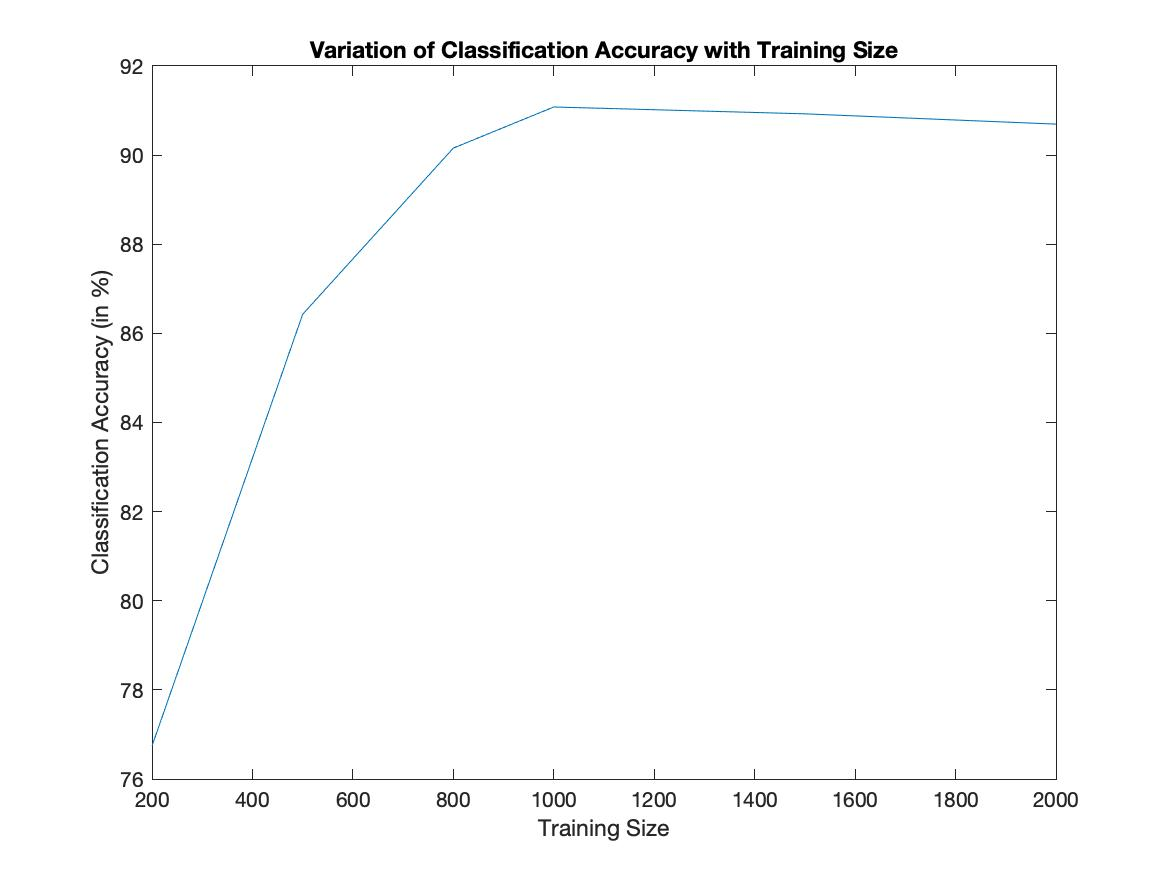
\includegraphics{Codes/Results/Logistic Train/Accuracy_Variance}
	\end{adjustbox}
	\caption{Variation of Classification Accuracy with the Number of Samples available for Training}
	\label{fig:accuracy_vs_trainsize}
\end{figure}

In addition to this, the confusion matrices for these experimentation were also plotted. The matrices are provided in \autoref{fig:log_reg_Confusion_Mat}. False postives are really crucial for spam email detection services. If an important mail gets marked as spam, it may be fatal for the users. So, classifcationa accuracy cannot be always used as a evaluation metric. The reason is that classification accuracy works on the total false cases and does not differentiate between false positives and false negatives. But, in some cases, false positives may be worse than false negatives. In case of spam email detection, that is the case. So, we should always check the confusion matrices to arrive at the final model based on the business aspect of the service. For this reason, the confusion matrices for the given experiments were checked and it was observed that $n=1000$ gives the least number of false positives as well. So, it can be considered as the best model provided by the experimentation.

\begin{figure}[H]
	\centering
	\begin{adjustbox}{width=0.9\paperwidth}
		\begin{tabular}{c c}
			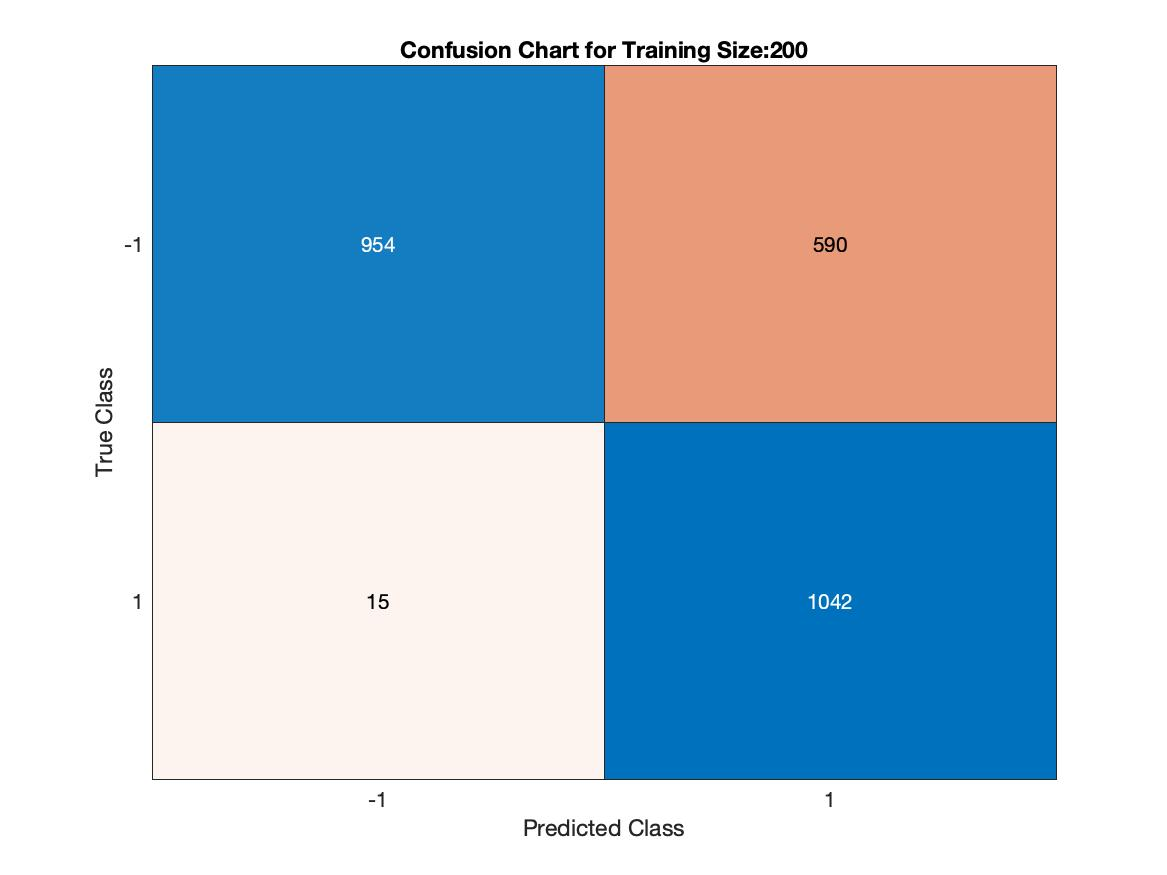
\includegraphics{Codes/Results/Logistic Train/Conf_Chart_Train_Size_200} & 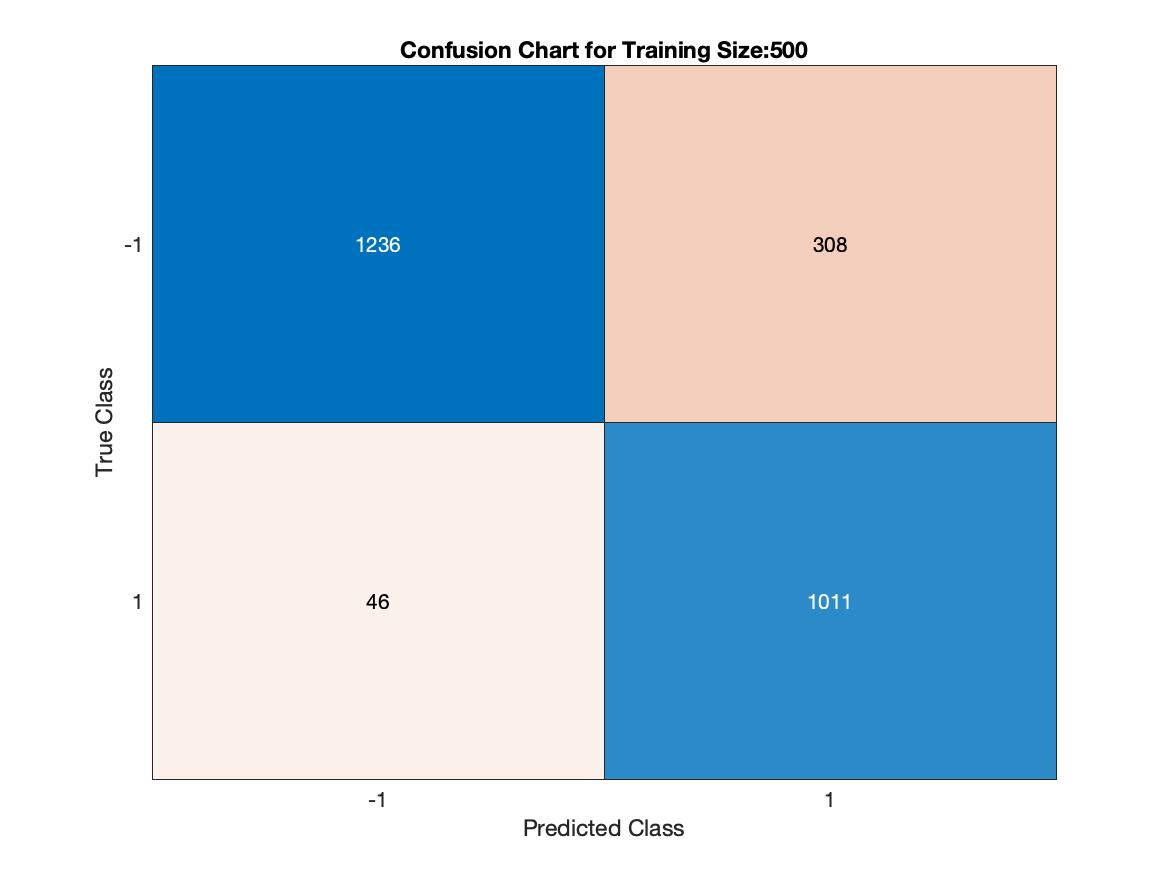
\includegraphics{Codes/Results/Logistic Train/Conf_Chart_Train_Size_500}\\ 
			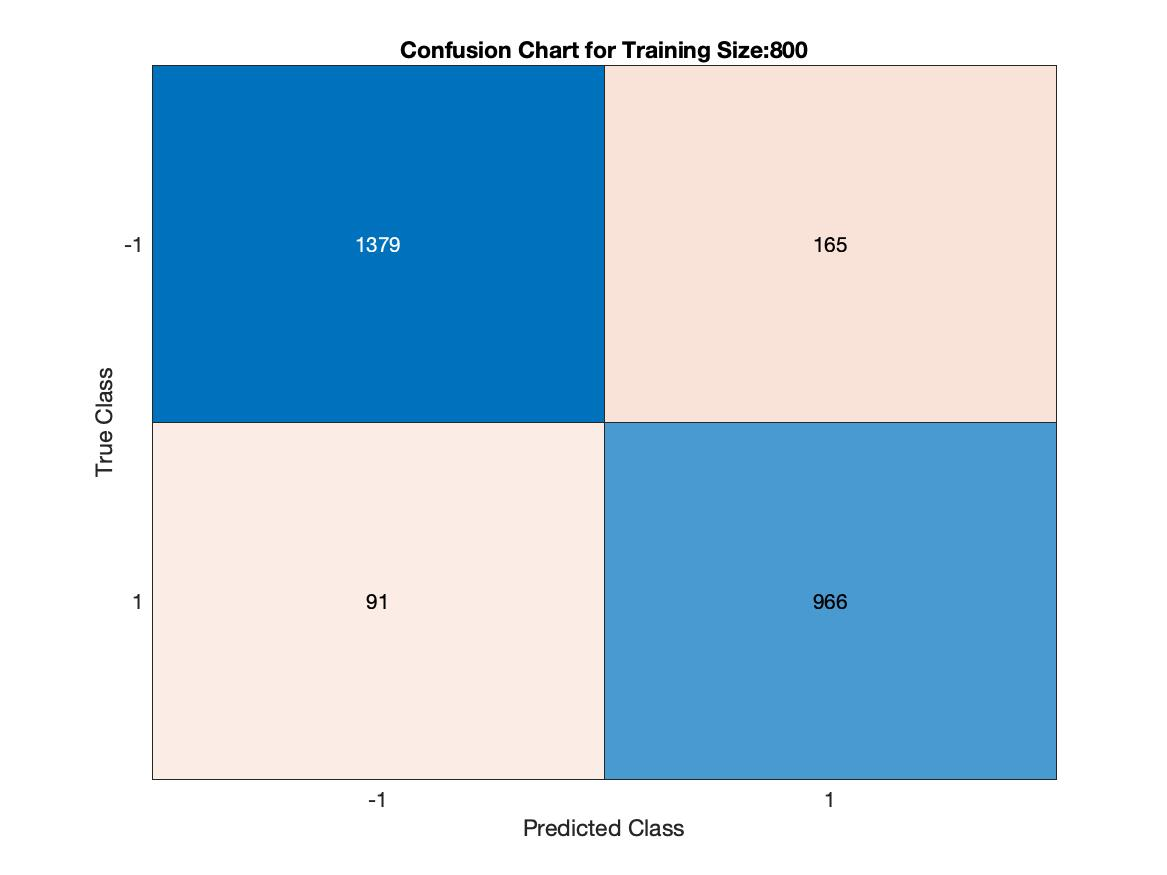
\includegraphics{Codes/Results/Logistic Train/Conf_Chart_Train_Size_800} & 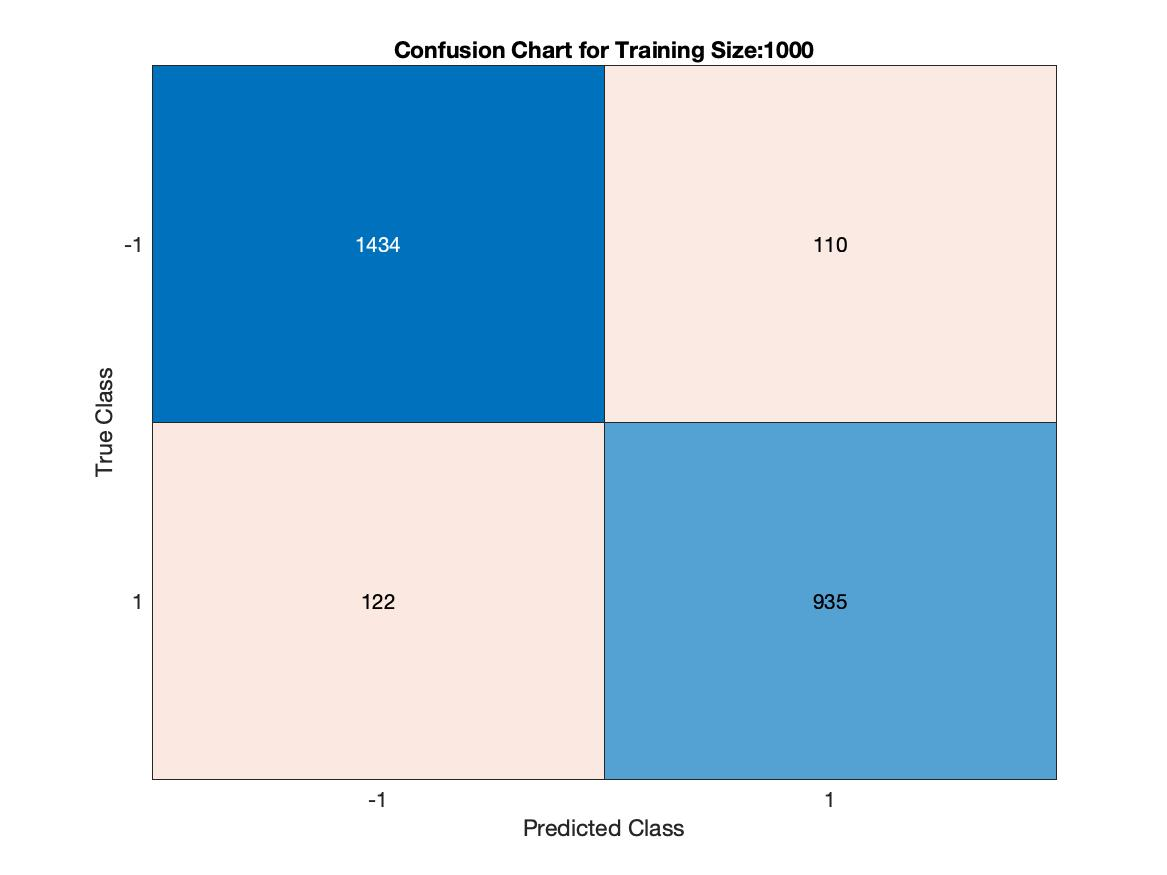
\includegraphics{Codes/Results/Logistic Train/Conf_Chart_Train_Size_1000}\\
			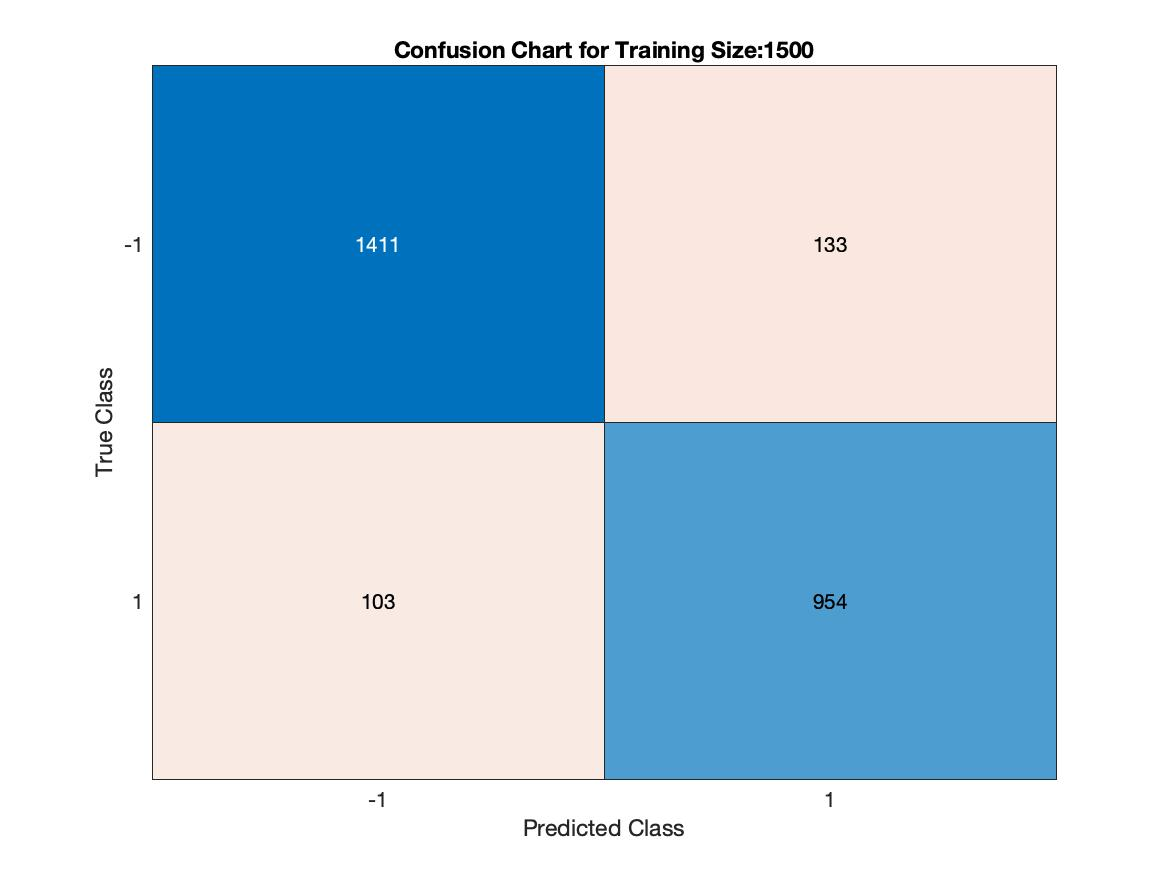
\includegraphics{Codes/Results/Logistic Train/Conf_Chart_Train_Size_1500} & 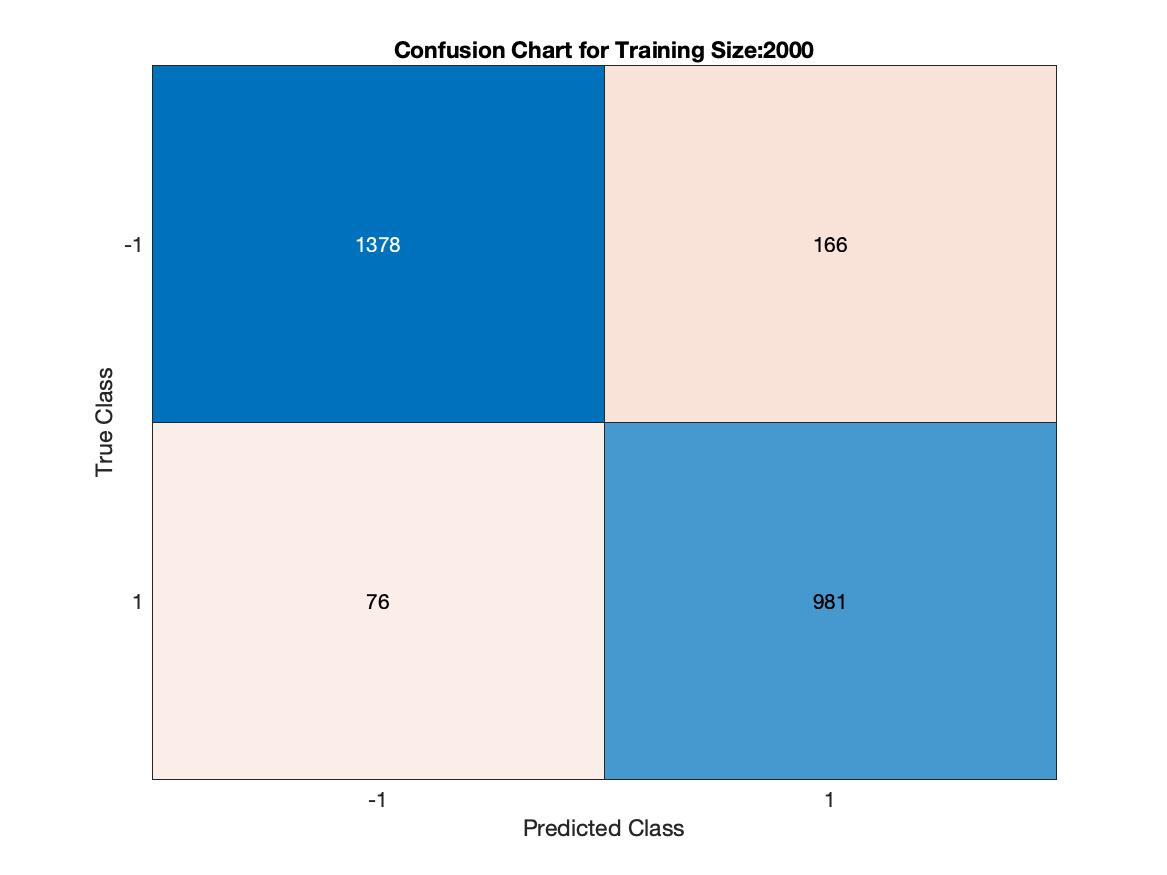
\includegraphics{Codes/Results/Logistic Train/Conf_Chart_Train_Size_2000}\\
		\end{tabular}
	\end{adjustbox}
	\caption{Plot of Confusion Matrices obtained for different training sizes}
	\label{fig:log_reg_Confusion_Mat}
\end{figure}

\section{\textbf{Sparse Logistic Regression: Experiment}}
The goal of this experiment is to add sparse regularization to the logistic regression framework and observe how it helps to reduce the number of features used for the classification (feature selection). For the simulation of the experimentation, \textit{\textbf{Alzheimers}} dataset is used as an application which is publicly available at: \href{https://github.com/jiayuzhou/CSE847/tree/master/data/alzheimers}{Alzheimers Dataset}.\\

The dataset is pre-divided into training and test samples. There are $172$ training samples and $74$ test samples in the dataset. Each sample has an associated label of either $+1$ (Alzheimer's Disease patient) or $-1$ (Mild Cognitive Impairment patient).  	

\subsection{Code}
The code used to implement the sparse logistic regression is presented below:
\lstinputlisting[language=Matlab]{Codes/logistic_l1_train.m}

\subsection{Experimental Outcome}

As a part of the experiment, the regularization parameters was varied as:\\ 
$par = 0.01, 0.1, 0.2, 0.3, 0.4, 0.5, 0.6, 0.7, 0.8, 0.9, 1$
Every different model was judged analyzed by $3$ imporant metrics: Classification Accuracy, AUC and Number of non-zero weights. $L1$-regularization leads to sparse models, so it is really interesting to see how change in the regularization parameter can lead to a change in the number of non-zero weights. As number of zero-weights increase in the model, the number of features used to build the classification model reduces. Thus $L1$-regularization helps to perform Feature Selection.\\

The result of the experimentation is presented in \autoref{fig:metric_scores} and \autoref{tab:metric_scores}. From the Figure, it can be observed that the number of non-zero weights decreases as the value of regularization parameter is increased. This means that the model is becoming more sparse with increase in the value of the parameter. On the other hand, it can be seen that accuracy is increasing as opposite to the variation in number of non-zero weights. This observation was pretty interesting. Particularly, in the later stages of the experimentation, the model was using only one non-zero weight and it was still giving almost $75\%$ accuracy. A careful look at the dataset made the idea clear. The test data consisted of imbalanced samples where approx. $75\%$ samples were having label $-1$. So, the model was simply classifying every sample to $-1$ and that is the reason why it was getting such a high accuracy using only $1$ feature. But it did not produce our intended model.\\

\begin{figure}[H]
	\centering
	\begin{adjustbox}{width=0.65\paperwidth}
			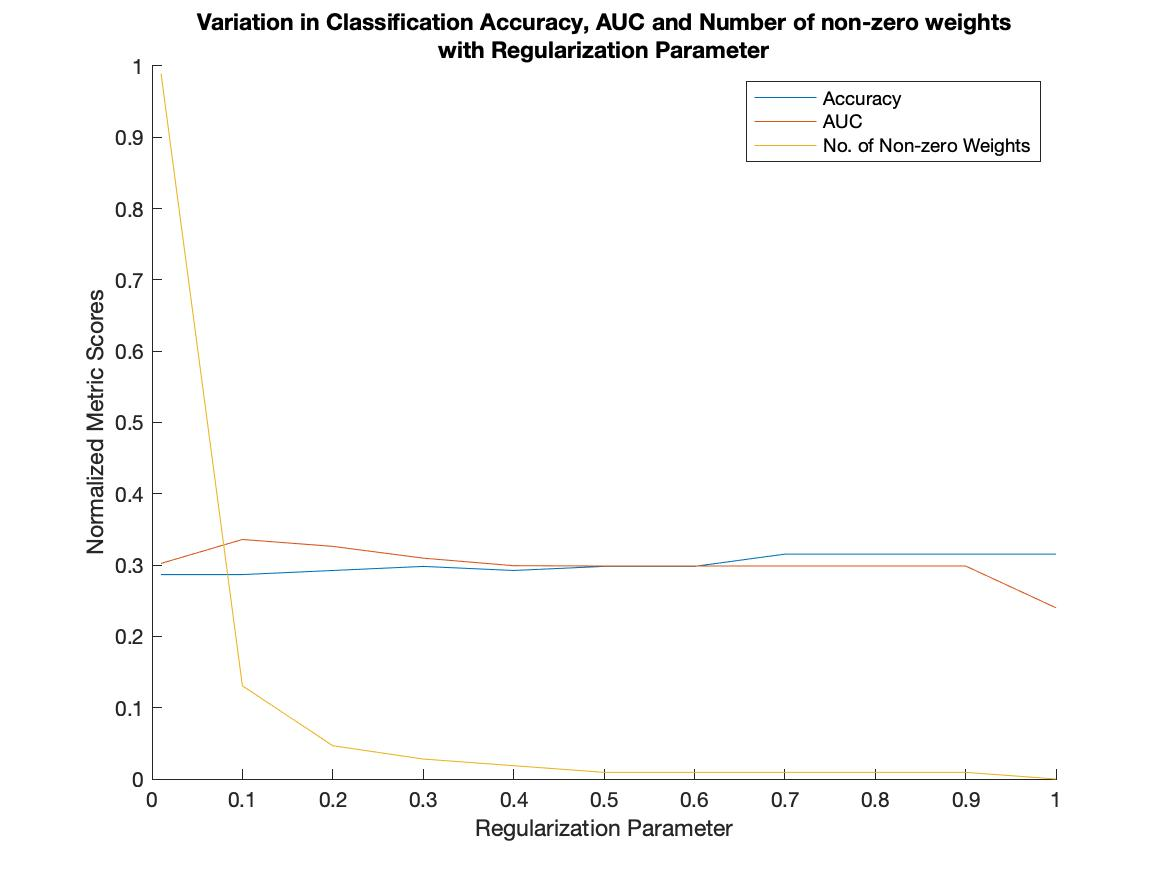
\includegraphics{Codes/Results/L1 Logistic Train/Metric_Variance} 
	\end{adjustbox}
	\caption{Plot of different metrics obtained for different values of regularized parameters}
	\label{fig:metric_scores}
\end{figure}


\begin{table}[H]
	\centering
	\begin{tabular}{|c|c|c|c|}
		\hline
		\textbf{Par} & \textbf{No. of Non-zero Weights} & \textbf{Accuracy} & \textbf{AUC} \\ \hline
		0.01 & 106 & 67.567568 & 0.629665 \\ \hline
		0.1 & 14 & 67.567568 & 0.699522 \\ \hline
		0.2 & 5 & 68.918919 & 0.679426 \\ \hline
		0.3 & 3 & 70.27027 & 0.644976 \\ \hline
		0.4 & 2 & 68.918919 & 0.622967 \\ \hline
		0.5 & 1 & 70.27027 & 0.62201 \\ \hline
		0.6 & 1 & 70.27027 & 0.62201 \\ \hline
		0.7 & 1 & 74.324324 & 0.62201 \\ \hline
		0.8 & 1 & 74.324324 & 0.62201 \\ \hline
		0.9 & 1 & 74.324324 & 0.62201 \\ \hline
		1 & 0 & 74.324324 & 0.5 \\ \hline
	\end{tabular}
	\caption{Different Metric Scores for different values of the regularization parameter}
	\label{tab:metric_scores}
\end{table}

In order to get some more insights to the problem, in the next stage, the confusion matrices for the experiments were plotted. The matrices are presented in \autoref{fig:log_l1_reg_Confusion_Mat}. After the parameter value reaches $0.7$, it starts assigning all the labels to $-1$, so there's no false negatives or true positives. Although it is able to achieve good classification accuracy, it is not a good model. For this reason, in case of imbalanced data, classification accuracy cannot serve as an appropriate metric. AUC (Area Under Curve) is a better metric compared to accuracy in such a scenario. Intuitioanlly, AUC denotes the probability of a model assigning higher value to a random positive example in comparison to a random negative example. In terms of AUC, the second model of the experimentation, i.e. parameter value of $0.1$, can be considered to be the best model out of all as it achieved the highest AUC score. 

\begin{figure}[H]
	\centering
	\begin{adjustbox}{width=0.8\paperwidth}
		\begin{tabular}{c c}
			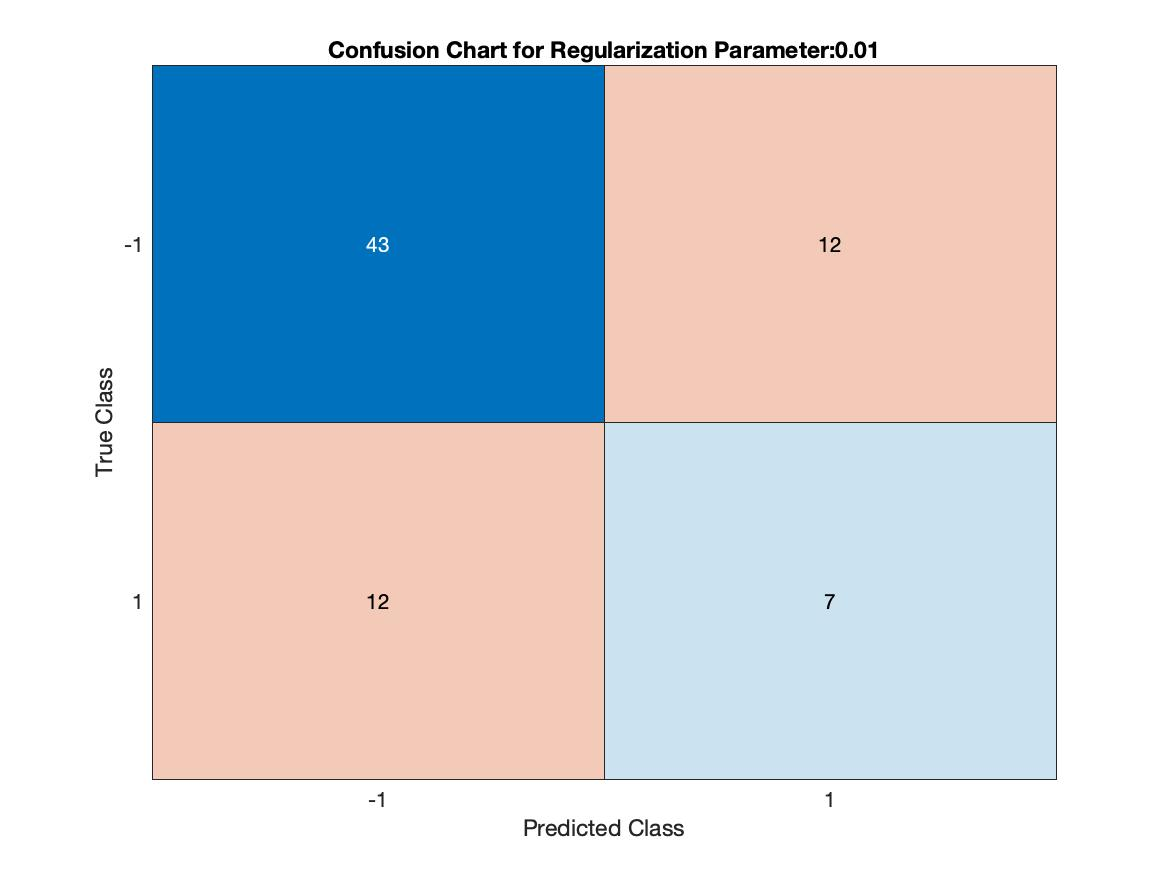
\includegraphics{Codes/Results/L1 Logistic Train/Conf_Chart_Reg_Par_0.01} & 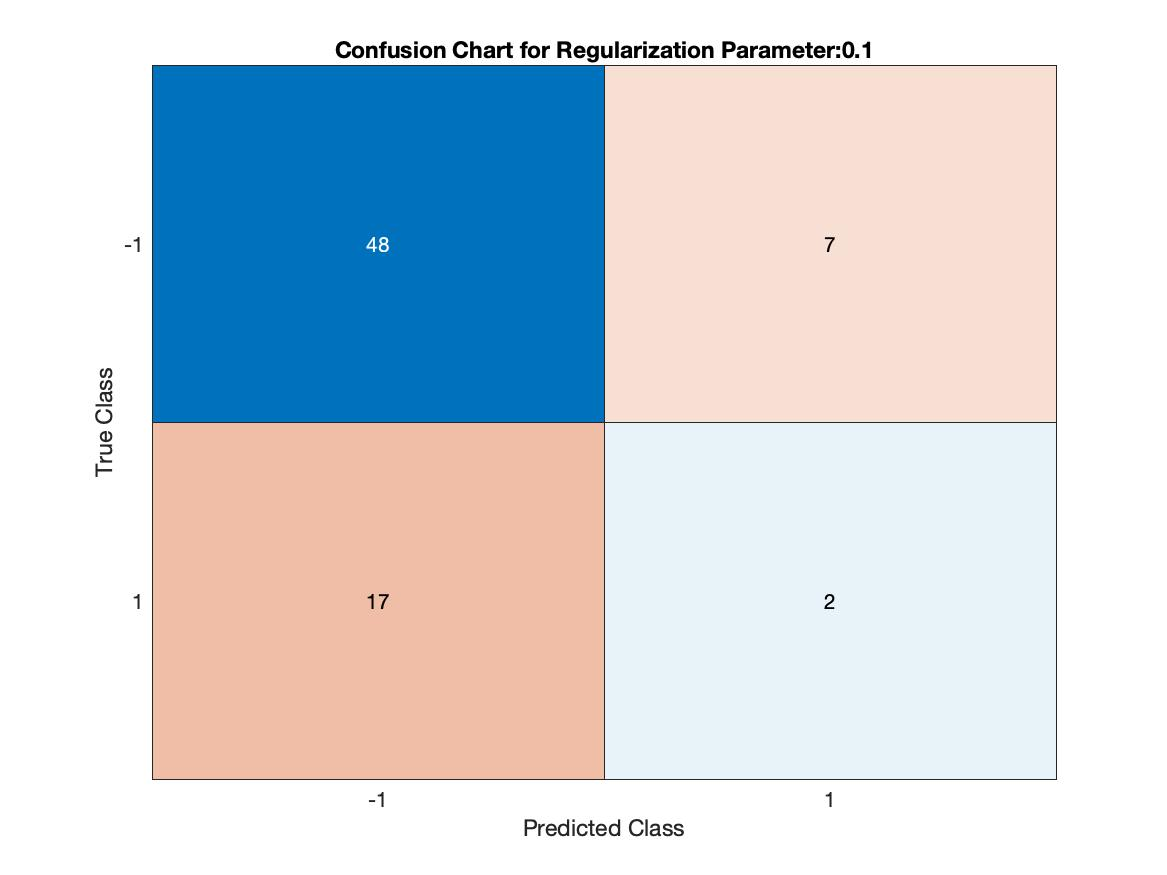
\includegraphics{Codes/Results/L1 Logistic Train/Conf_Chart_Reg_Par_0.1}\\ 
			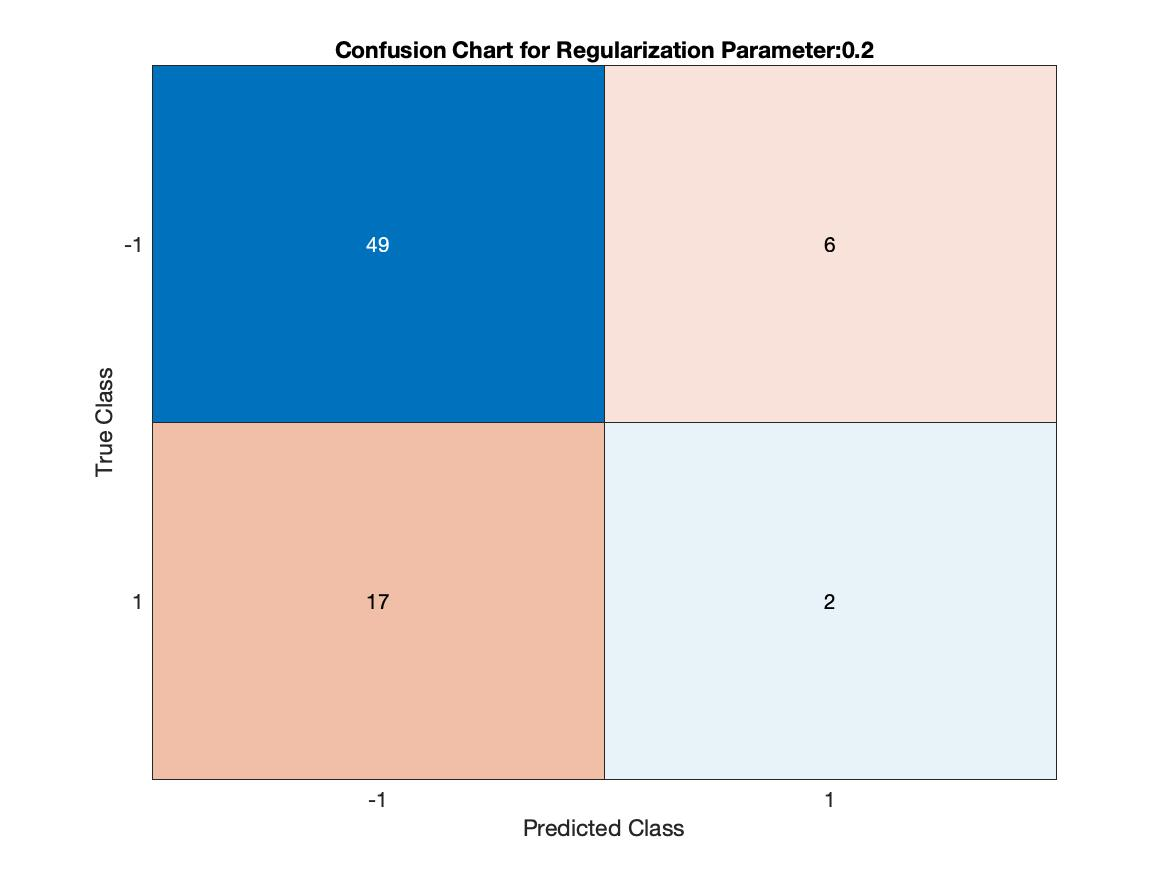
\includegraphics{Codes/Results/L1 Logistic Train/Conf_Chart_Reg_Par_0.2} & 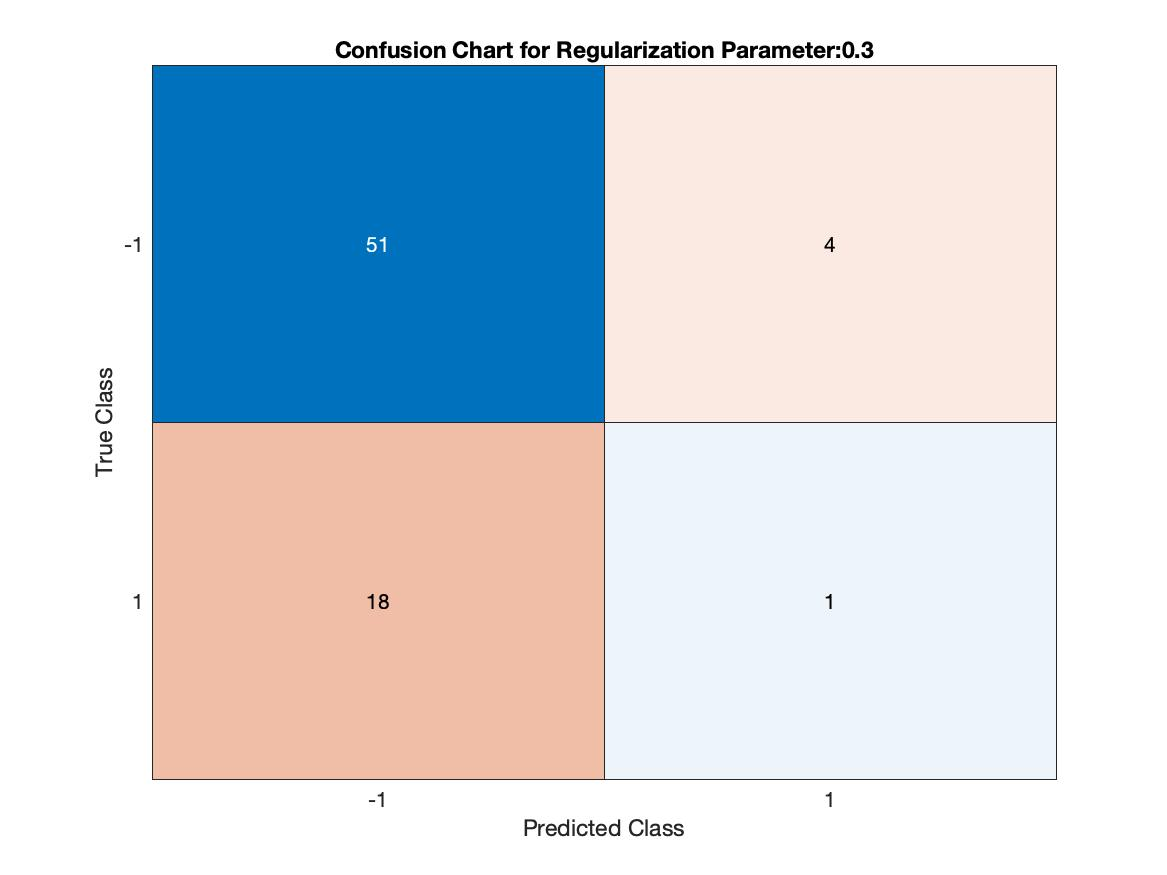
\includegraphics{Codes/Results/L1 Logistic Train/Conf_Chart_Reg_Par_0.3}\\
			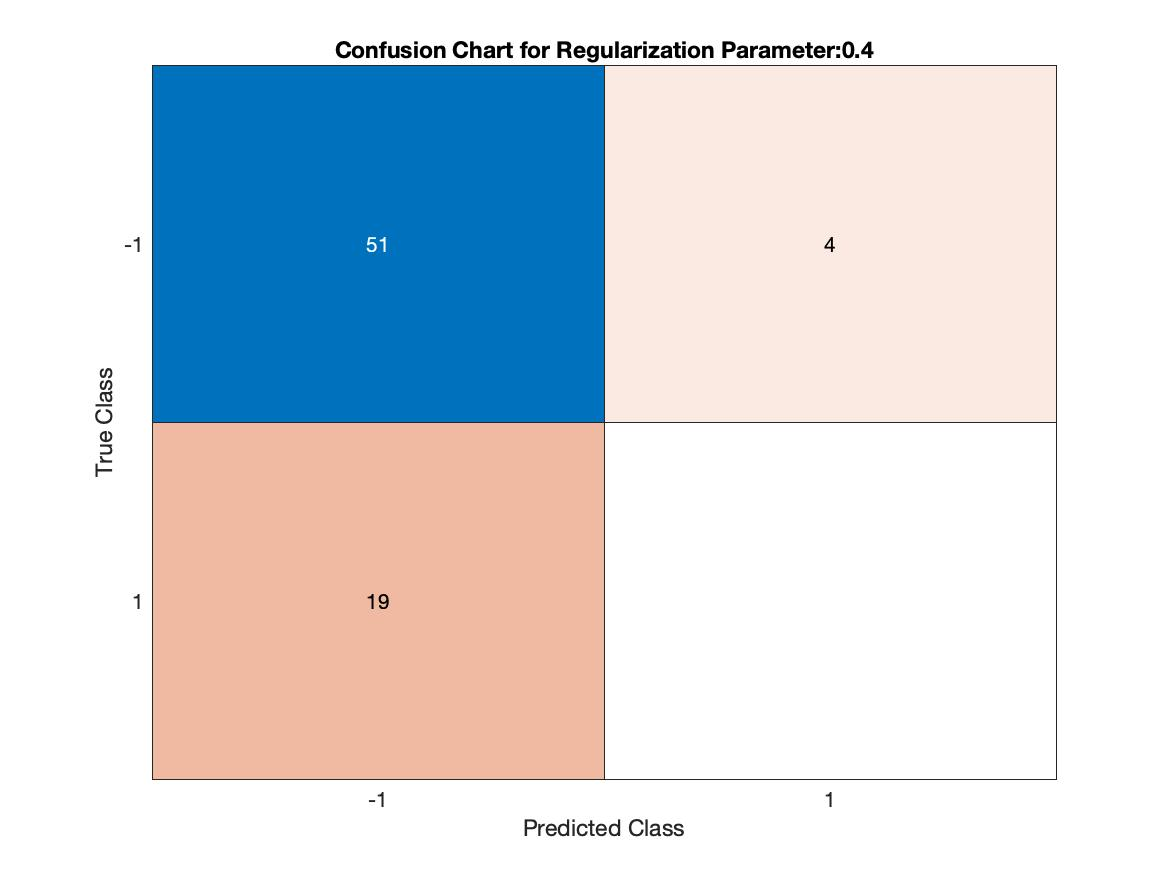
\includegraphics{Codes/Results/L1 Logistic Train/Conf_Chart_Reg_Par_0.4} & 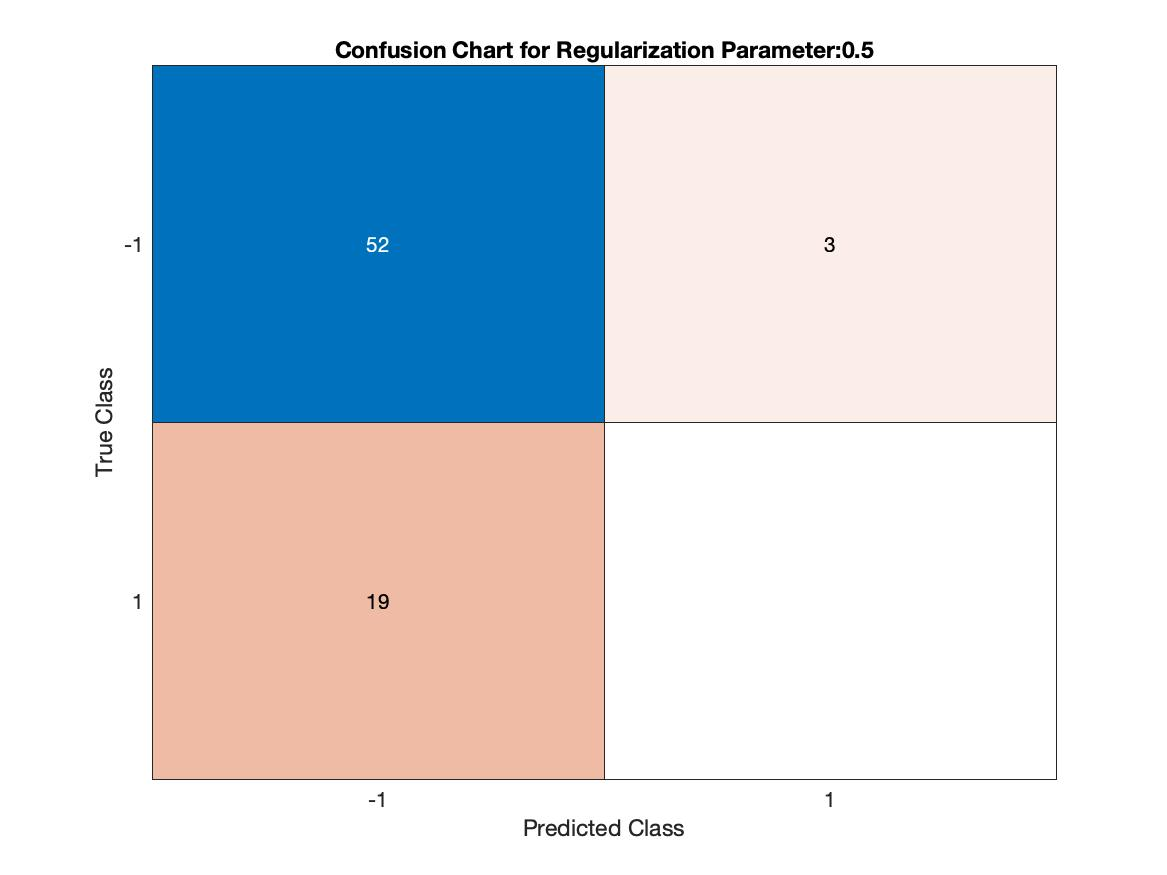
\includegraphics{Codes/Results/L1 Logistic Train/Conf_Chart_Reg_Par_0.5}\\
			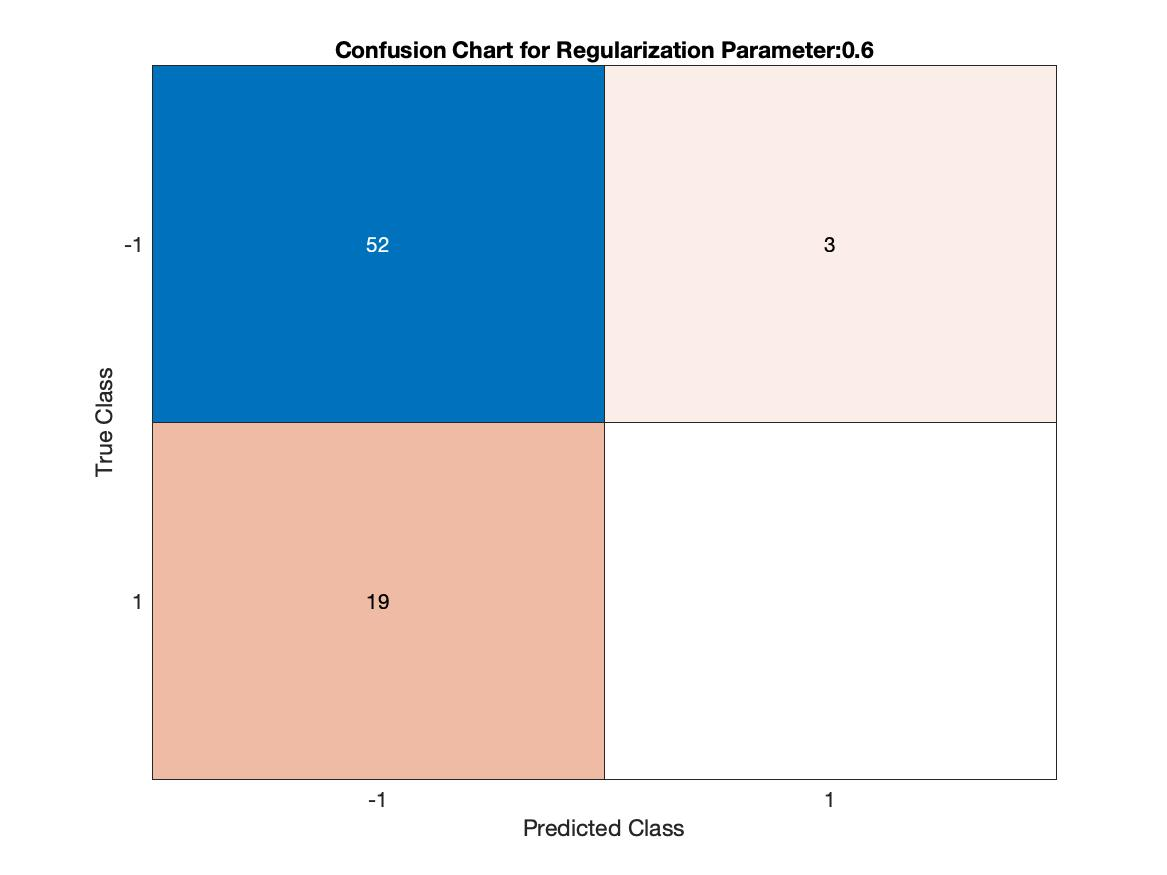
\includegraphics{Codes/Results/L1 Logistic Train/Conf_Chart_Reg_Par_0.6} & 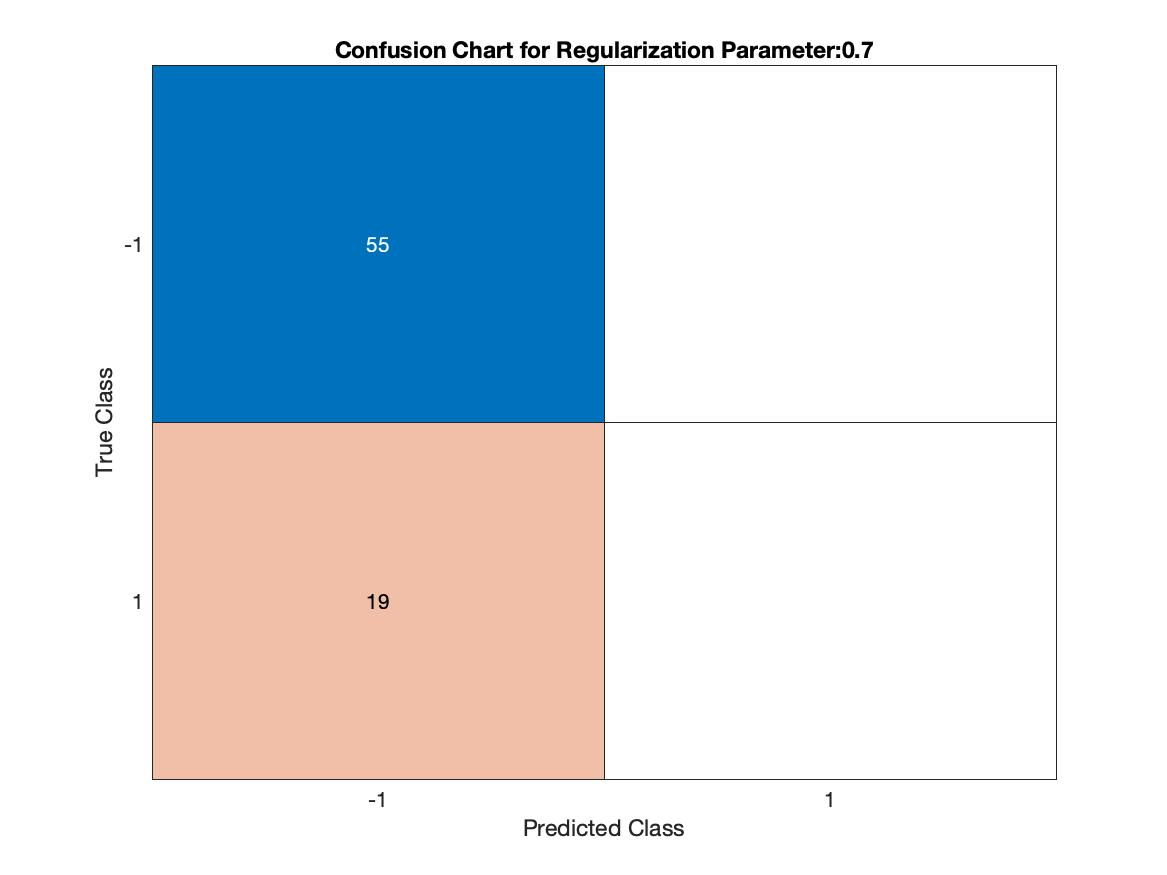
\includegraphics{Codes/Results/L1 Logistic Train/Conf_Chart_Reg_Par_0.7}\\
		\end{tabular}
	\end{adjustbox}
	\caption{Plot of Confusion Matrices obtained for different values of the Regularization Parameter}
	\label{fig:log_l1_reg_Confusion_Mat}
\end{figure}

\end{document}
